%%%%%%%%%%%%%%%%%%%%%%%%%%%%%%%%%%%%%%%%%%%%%%%%%%%%%%%%%%%%
%%% APPENDICES
%%%%%%%%%%%%%%%%%%%%%%%%%%%%%%%%%%%%%%%%%%%%%%%%%%%%%%%%%%%%

\documentclass[12pt,letterpaper]{article}
\usepackage[top=0.85in,left=0.75in,footskip=0.75in]{geometry}
\usepackage{amsmath,amssymb}



% Use adjustwidth environment to exceed column width (see example table in text)
\usepackage{changepage}

% Use Unicode characters when possible
\usepackage[T2A]{fontenc}
\usepackage[utf8x]{inputenc}

\usepackage{easyeqn}
\usepackage{algorithm}
\usepackage{algorithmic}

\usepackage{float}

% textcomp package and marvosym package for additional characters
\usepackage{textcomp,marvosym}

% cite package, to clean up citations in the main text. Do not remove.
\usepackage{cite}

% Use nameref to cite supporting information files (see Supporting Information section for more info)
\usepackage{nameref,hyperref}

% line numbers
\usepackage[right]{lineno}

% ligatures disabled
\usepackage{microtype}
\DisableLigatures[f]{encoding = *, family = * }

% color can be used to apply background shading to table cells only
\usepackage[table]{xcolor}

% array package and thick rules for tables
\usepackage{array}

\usepackage{graphicx}
\begin{document}

\section{Significantly different words}
\begin{enumerate}
    \item Top 10 Russian words in which the number of hits in VLPFC (online encoding) and Sham groups is significantly different (higher or lower) from other words:
    \textbf{аудитория (auditorium), динозавр (dinosaur), дождь (rain), лектор (lecturer), паук (spider), политик (politican), почта (post), священник (priest), шея (neck), шмель (drone).}
    \item Top-10 Russian words in which the number of False Alarms in VLPFC and Sham groups is significantly different (higher or lower) from other words: \newline
    VLPFC: \textbf{балерина (ballerina), журавль (crane), тигр (tiger), почта (post), павлин (peacock), аудитория (auditorium), лектор (lecturer), пирамида (pyramid),}\newline \textbf{ осьминог (octopus), бухгалтер (accountant). пирамида, осьминог, бухгалтер.}\newline
    Sham: \textbf{фотограф (photograph), сеть (network), змея (snake), тигр (tiger), тюлень (seal), каток (slide), шмель (drone), повар (cook), узел (knot), свинья (pig).}
    \item The top-10 list of Russian & English words which are differently remembered based on ROC analysis: \newline
    Russian: \textbf{волк (wolf), кукла (doll), гитарист (guitarist), павлин (peacock), доктор (doctor), карман (pocket), туалет (toilet), психолог (psychologist), политик (politician), крыша (roof).} \newline
    English: \textbf{athlete, politician, whiskey, skirt, drone, galaxy, infection, doctor, philosopher, astronaut.} 
    \item The top-10 list of Russian & English words with higher Reaction Time:\newline
    Russian: \textbf{галактика (galaxy), паломник (pilgrim), прачечная (laundry), челюсть (jaw), котенок (kitten), петиция (petition), выходной (weekend), соловей (nightingale), инфекция (infection), аптекарь (pharmacist).} \newline
    English: \textbf{kidney, shelter, monument, snail, essay, fingerprint, petition, clown, pheasant, jumper.}
    \item The top-10 list of Russian & English words with lower Reaction Time: \newline
    Russian: \textbf{пилот (pilot), сеть (network), озеро (lake), палец (finger), робот (robot), дельфин (dolphin), акула (shark), зомби (zombie), чернила (ink), праздник (party).} \newline
    English: \textbf{prize, lotion, duck, skirt, graveyard, bubble, quiz, beach, roof, drone.}
    
\newpage

\section{Data Augmentations}
To artificially enlarge the training set for our trials, we use the augmentation procedure proposed in the paper ``Word embedding perturbation for sentence classification'' by Dongxu Zhang and Zhichao Yang. We multiply each word vector by a random noise of the same shape element-wise:
\begin{equation}
    X_{aug} = X \odot Z,
\end{equation}
where \(Z\) has the same shape as \(X\) and is sampled from \(N(\mu=1, \sigma=0.1)\). For the example of augmentation consult Figure~\ref{fig:augmentation} below.

\begin{figure}[h!]
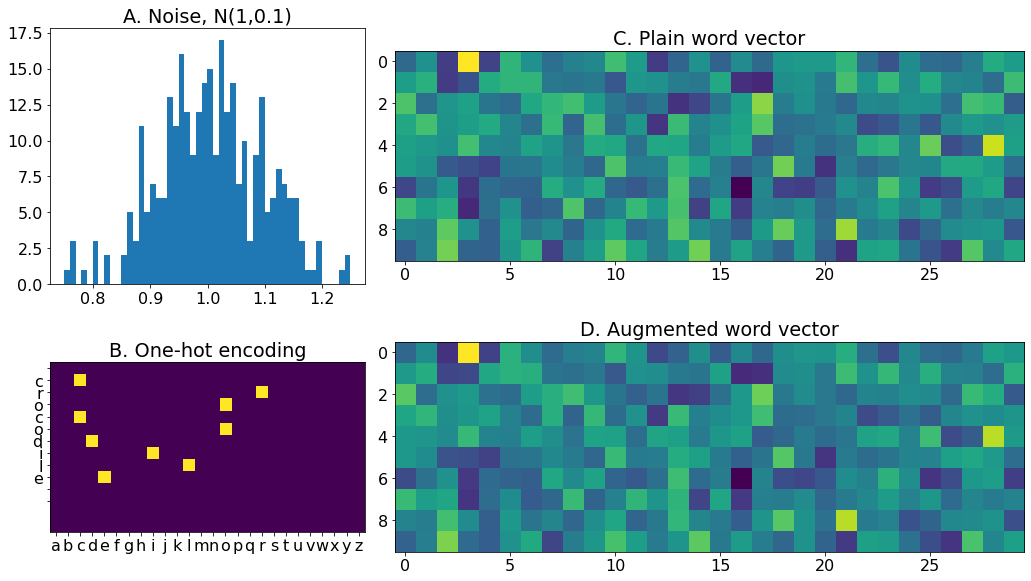
\includegraphics[width=\textwidth]{figures/Appendix2.png}
\caption{A. The noize we multiply our word vectors by. At B. we show the one-hot encoding of the word ``crocodile''. At C. you can see plain word vector and D. shows the augmented word vector for the same word, ``crocodile''. We reshape the vector of dimensionality 300 to a matrix of shape (10,30) to visualize. The result of augmentation is mostly the same vector with some values enhanced and some diminished. }
\label{fig:augmentation}
\end{figure}
In case of AUROC regression we also multiply the labels by a random number sampled from uniform distribution with lower bound of 0.9 and upper bound of 1.1. We run augmentation three times and combine the augmented and plain data to form the training set. The test set remains without augmentation.

\newpage

\section{Participant-Independent ML Trials}


\begin{table}[h!]
\centering
\caption{The performance of participant-independent TPOT models.}
\begin{tabular}{|l|r|r|r|r|} \hline
trial &  train SCC &  train SCC p-value &  test SCC &  test SCC p-value \\ \hline
Both, word vectors &   0.99 &       0 & -0.05 &          0.61 \\ \hline
English word vectors &   0.99 &      0 &  0.13 &          0.36 \\ \hline
English, one-hot encoding &   0.99 &      0 &  0.02 &          0.91 \\ \hline
Russian word vectors &   0.97 &      0 &  0.08 &          0.59 \\ \hline
Russian word vectors &   0.98 &      0 &  0.18 &          0.22 \\ \hline
\end{tabular}

\end{table}

\begin{figure}[h!]
\centering
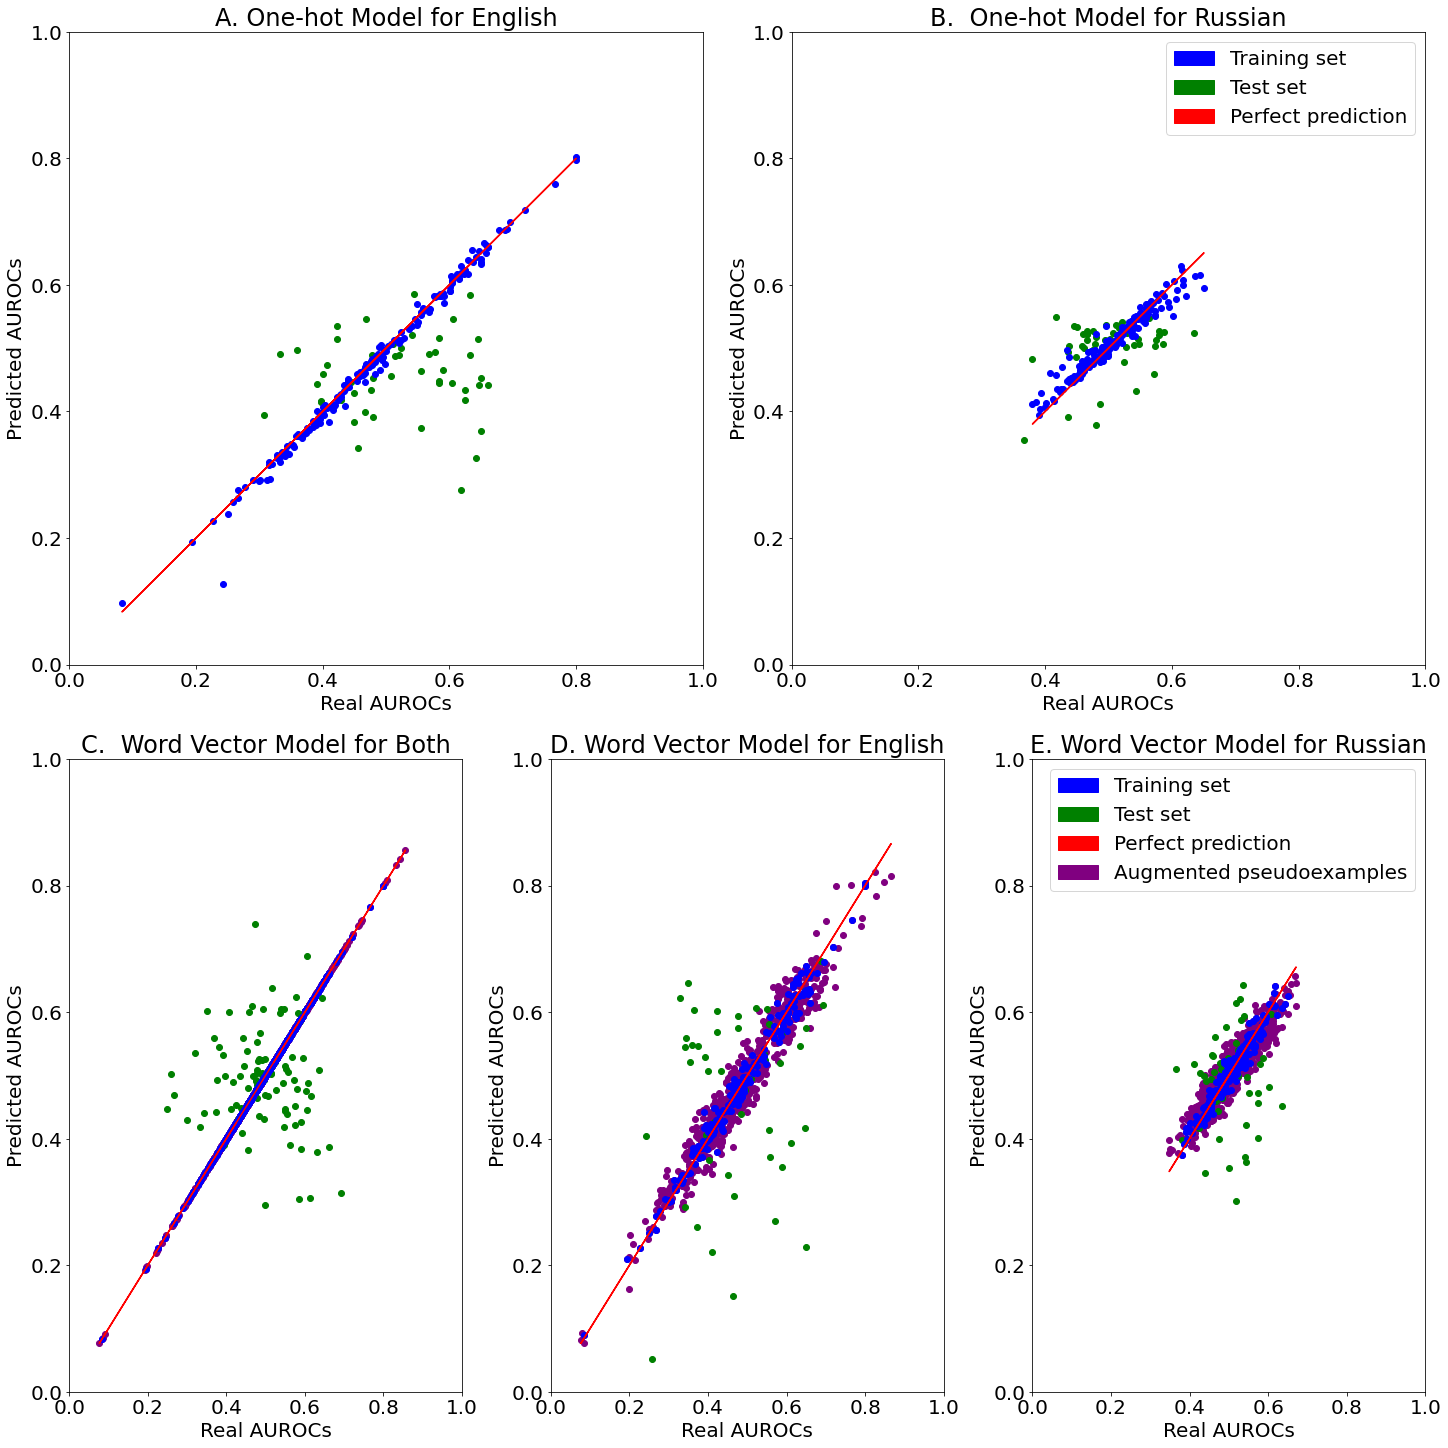
\includegraphics[width=0.8\linewidth]{figures/Appendix3.png}
\caption{The prediction plots for one-hot encoding-based model for English (A) and Russian (B) words shows clear lack of generalization ability. We were able to overfit our AutoPyTorch model for the training set. Same follows for word vector-based models for both English and Russian words combined (C), only English (D) and only Russian (E).
}
\end{figure}

\newpage
\section{Participant-Dependent ML Trials}

\begin{table}[h!]
\centering

\caption{The performance of participant-dependent AutoPyTorch models based on one-hot encoding. Most of the times the performance is very poor both in the training and testing set. We were unable to fit a good model for each pariticpants, we didn't even get it to overfit the training set.}
\begin{tabular}{|l|r|r|}
\hline
trial &  train AUROC \(\pm\) std &  test AUROC \(\pm\) std \\
\hline
Russian All &    0.50 \(\pm\)   0.01 &   0.50 \(\pm\)  0.02 \\ \hline
Russian Sham &    0.50 \(\pm\)   0.01 &   0.50 \(\pm\)  0.02 \\ \hline
Russian VLPFC &    0.50 \(\pm\)   0.00 &   0.50 \(\pm\)  0.01 \\ \hline
Russian DLPFC Offline &    0.50 \(\pm\)   0.02 &   0.51 \(\pm\)  0.03 \\ \hline
Russian DLPFC Online &    0.50 \(\pm\)   0.00 &   0.50 \(\pm\)  0.02 \\ \hline
English All &    0.50 \(\pm\)   0.0 &   0.50 \(\pm\)  0.01 \\ \hline
English Sham &    0.50 \(\pm\)   0.00 &   0.50 \(\pm\)  0.01 \\ \hline
English VLPFC &    0.50 \(\pm\)   0.00 &   0.50 \(\pm\)  0.01 \\ \hline
\end{tabular}
\end{table}

\begin{table}[h!]
\centering
\caption{The performance of participant-dependent TPOT models based on FastText word vectors. The performance is rather poor on the testing set. Unlike the models based on one-hot encoded models, we were able to overfit them on the training set with 10-fold crossvalidation, but the generalization ability remained very low.}
\begin{tabular}{|l|r|r|}
\hline
trial &  train AUROC \(\pm\) std &  test AUROC \(\pm\) std \\ \hline
Russian All &         1.0 \(\pm\) 0.0 &   0.51 \(\pm\)  0.07 \\ \hline
Russian Sham &         1.0 \(\pm\)    0.0 &   0.52 \(\pm\)  0.07 \\ \hline
Russian VLPFC &         1.0 \(\pm\)  0.0 &   0.50 \(\pm\)  0.07 \\ \hline
Russian DLPFC Offline &         1.0 \(\pm\)   0.0 &   0.54 \(\pm\)  0.08 \\ \hline
Russian DLPFC Online &         1.0 \(\pm\)  0.0 &   0.51 \(\pm\)  0.06 \\ \hline
English All &         1.0 \(\pm\)  0.0 &   0.47 \(\pm\)  0.07 \\ \hline
English Sham &         1.0 \(\pm\)    0.0 &   0.47 \(\pm\)  0.07 \\ \hline
English VLPFC &         1.0 \(\pm\)        0.0 &   0.47 \(\pm\)  0.07 \\ \hline
\end{tabular}
\end{table}


\end{document}